% Using KOMA Script document style
% Font size setting and
% option to skip empty lines as new paragraphs
\documentclass[10pt,a4paper]{article}
\usepackage{silence}
\WarningFilter{latex}{Command}
% Packages without Options
\usepackage{
	mathtools,
	array,
	amsfonts,
	amssymb,
	geometry,
	enumitem,
	venndiagram,
	booktabs,
	tikz,
	interval,
	makecell,
	textcomp,
	gensymb,
	float,
	pgfkeys,
	pgfplots,
	wrapfig,
	lipsum,
	karnaugh-map,
	footnote,
	tablefootnote,
	xcolor,
	longtable,
	subcaption,
	algorithm,
	algpseudocode,
	pdfpages,
    nicematrix,
    sectsty,
    titlecaps,
	listings,
	minted,
	wrapfig,
}

\definecolor{mintedbackground}{rgb}{0.97,0.97,0.97}

\setminted[cpp]{
bgcolor=mintedbackground,
    linenos=true,
    breaklines=true,}

\setminted[python]{
bgcolor=mintedbackground,
    linenos=true,
    breaklines=true,}
    
% Enforce title case for section
% \allsectionsfont{\titlecap}

% \lstset{basicstyle=\footnotesize\ttfamily,breaklines=true}

\linespread{1.5}

% Packages with Options
\usepackage[british]{babel} 
\usepackage[framemethod=tikz]{mdframed}
\usepackage[colorlinks,linkcolor=cyan, citecolor=cyan, urlcolor=cyan]{hyperref}
\usepackage[labelfont=bf,textfont=it,labelsep=period]{caption}
\usepackage[RPvoltages]{circuitikz}

% Package: Interval
% Sets the style of mathematical intervals
\intervalconfig{
soft open fences, separator symbol=,,
}

% Package: Geometry
% Sets the page margins
\geometry{
    a4paper,
    left=32mm,
    right=22mm,
    top=22mm,
    }
	
% Creates a proper caption name for algorithms
\newcommand{\algorithmautorefname}{Algorithm}
\newcommand{\listingautorefname}{Listing}
\algrenewcommand{\algorithmiccomment}[1]{\texttt{// #1} }
% Creates a numbered environment for Theorems
\newtheorem{theorem}{Theorem}

% Redefine the implication arrow to be a simple, thin arrow instead of the default, thick arrow
\renewcommand{\implies}{\rightarrow}

% Create a new command for the set complement to make my logical statements easier to read
\newcommand{\compl}{\overline}

% Creates commands for combinatorics nCr and nPr
\newcommand{\nCr}[2]{\,_{#1}C_{#2}} % nCr
\newcommand{\nPr}[2]{\,_{#1}P_{#2}} % nPr

% Package: tikz
% Loads libraries for drawing automata, 
\usetikzlibrary{automata,positioning,shadows,arrows, shapes.gates.logic.US, calc}

% Creates a command to create a button shape
\newcommand*\keystroke[1]{%
  \tikz[baseline= (key.base)]
    \node[%
      draw,
      fill=white,
      drop shadow={shadow xshift=0.25ex,shadow yshift=-0.25ex,fill=black,opacity=0.75},
      rectangle,
      rounded corners=2pt,
      inner sep=1pt,
      line width=0.5pt,
      font=\scriptsize\sffamily
    ] (key) {#1\strut};
}

% Package: pgfplot
% Sets the global options for PGF Plots
\pgfplotsset{compat=newest}

% Package: tikz
% Flowchart Shapes
\tikzstyle{startstop} = [rectangle, rounded corners, minimum width=3cm, minimum height=1cm,text centered, draw=black, fill=red!30]
\tikzstyle{io} = [trapezium, trapezium left angle=70, trapezium right angle=110, minimum width=3cm, minimum height=1cm, text centered, draw=black, fill=blue!30]
\tikzstyle{process} = [rectangle, minimum width=3cm, minimum height=1cm, text centered, draw=black, fill=orange!30]
\tikzstyle{decision} = [diamond, minimum width=3cm, minimum height=1cm, text centered, draw=black, fill=green!30]
\tikzstyle{arrow} = [thick,->,>=stealth]

% Disable Minted syntax error highlights (red boxes)
\AtBeginEnvironment{minted}{%
  \renewcommand{\fcolorbox}[4][]{#4}} %Adjust this based on where your Summary is stored
\title{CM2020: Agile Software Projects \\ Midterm Report, Group 6 (Tutor Group 1)}
\author{Arjun  Muralidharan}
\graphicspath{{./images/}}
\begin{document}


\maketitle
\newpage
\tableofcontents
\listoffigures
%\listoftables
% \listofalgorithms
\listoflistings
\newpage
\renewcommand{\subsubsectionautorefname}{section\negthinspace}

\section{Aims and Objectives}
\subsection{Background and problem}
As most college students would testify, motivation to study hard is a scarce resource and one that can easily get depleted. Any technique or tool that can increase motivation can provide great value to students and to the educational system in general. In addition, students with a growth mindset Students that have growth mindset compete with themselves, constantly looking for new ways to study smarter and improve both efficiency and effectiveness of their study. 

By their nature, most grading systems in education, as assessments of student academic achievement, are means for ranking students. Today’s connected and highly technological environment provides the opportunity to use gamification to increase motivation of students. 

Every module in a degree program is different and may require tailored strategy for study. Reflecting on a completed module provides “hindsight 20/20” notes on what worked well and what can be improved. In a collaborative environment however, students are not limited to their own experiences - they can benefit from wisdom and experience of fellow students.

\subsection{Aim and Value Proposition}
Our aim is to motivate the students to be their best selves and adopt the life-long growth mindset.

For college students that need extra motivation and study strategies, our "wisdom leaderboard" app will provide the rankings against other students and their notes.

We hope that this would lead to better academic achievements and adoption of empirical approach to lifelong self-improvement.

In order for the app to fulfill the aim and make a meaningful impact in the world, it needs to be actively used by many students. We therefore need to make the app accessible, easy to use and engaging to the widest possible population of students.

\subsection{Usability Goals}

\subsection{Measuring Success}
\textit{This section should set out the measuring criteria for your work and your presentation will be judged in relation to these aims and objectives.}

\section{Market Research}
Initial desk research indicates that the selected project, a grades leaderboard, does not have a direct competitor. There are some utilities which partially solve the problem we are tackling - namely, tracking grades - but none of these enable the user to compare themselves to their peers, nor aggregates grade data. As such, we must cast a wide net to analyze our place in the market and consider \emph{alternative solutions}. We have identified utilities which overlap with our project in terms of possible user needs as well as tools which solve analogous problems in different domains in order to get a more comprehensive picture of where our product stands in the market.
\subsection{Overview of Alternative Solutions}
Our solution offers two mains functions: \textbf{tracking grades} and \textbf{sharing/comparing} grades. For each feature, we have documented the alternative solutions, their specific functionality and notable design choices.
\subsubsection{Grade Tracking}
We surveyed various existing tools that enable students to track grades. Some peer-created utilities and University of London portal were discovered through our teammates' participation in this course, while \texttt{gpacalculator.io} \cite{gpa_calculator} is an example of many similar utilities that were found by searching 'grade tracking' and 'grade calculator' in a web search.

\paragraph{Peer student's Python command line grade calculator}
A peer student within the BSc Computer Science program at University of London developed a command line grades calculator \cite{lavoie_2020}. Users record their grades in a JSON file and run the script from the command line to see grade and other relevant information, as shown in \autoref{fig:py-calc}.

\begin{figure}[H]
\noindent 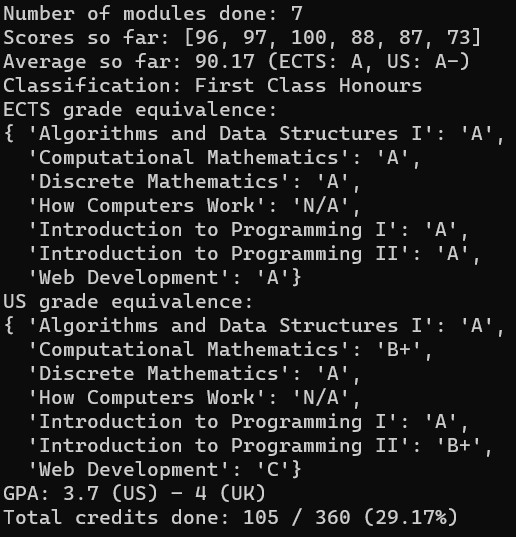
\includegraphics[height=200pt]{py-example-output.jpg}
\centering
\caption{Python Calculator Sample Output}
\label{fig:py-calc}
\end{figure}

\subparagraph{Notable Features}
The tool allows tracking course-level and cumulative grades and converts to ECTS (Europe) and US scales. It also support conversion from US to UK GPA scores and determines which classification your grades fall into. Further, it allows tracking how many credits out of 360 were completed.

\subparagraph{Notable Design Choices}
The design is lightweigth as it can be installed locally and run from a command line. The input is provided via a JSON file, which also allows easily storing, versioning and sharing a set of grades.

\paragraph{Peer's Google Sheets Degree Planner}
Another student (and co-author of this paper) have published a spreadsheet-based tool to track and calculate grades \cite{muralidharan_2020}. Users records their grades in a Google sheet to track their credits and grades, as shown in \autoref{fig:deg-planner}.
\begin{figure}[H]
\noindent 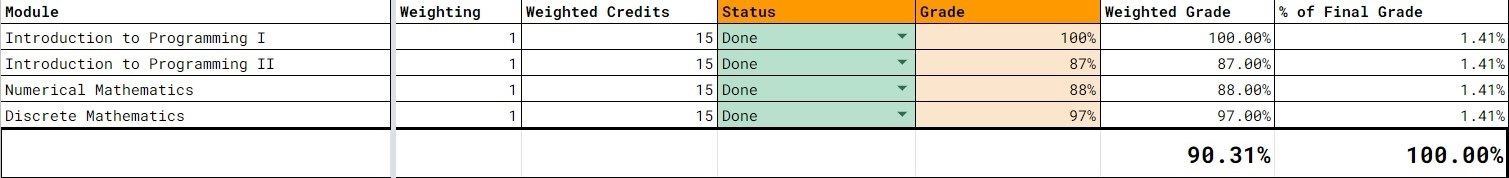
\includegraphics[width=\textwidth]{degree-planner-partial}
\centering
\caption{Google Sheets Degree Planner Excerpt}
\label{fig:deg-planner}
\end{figure}

\subparagraph{Notable Features}
The tool allows tracking course-level and cumulative grades, allows tracking how many credits out of 360 were completed and also highlights which modules are optional. It allows planning modules across semesters in order to distribute the courseload.

\subparagraph{Notable Design Choices}
This tool is implemented with Google Sheets, which makes it easier to use for many people, and allows easy sharing of the tool as anyone has free access to the software without any local installation.

\paragraph{gpacalculator.io}

A publicly available website, GPA Calculator \cite{gpa_calculator}, allows users to enter their grades in a web form and see cumulative results, converted to various other grading standards.

\begin{figure}[H] 
\noindent 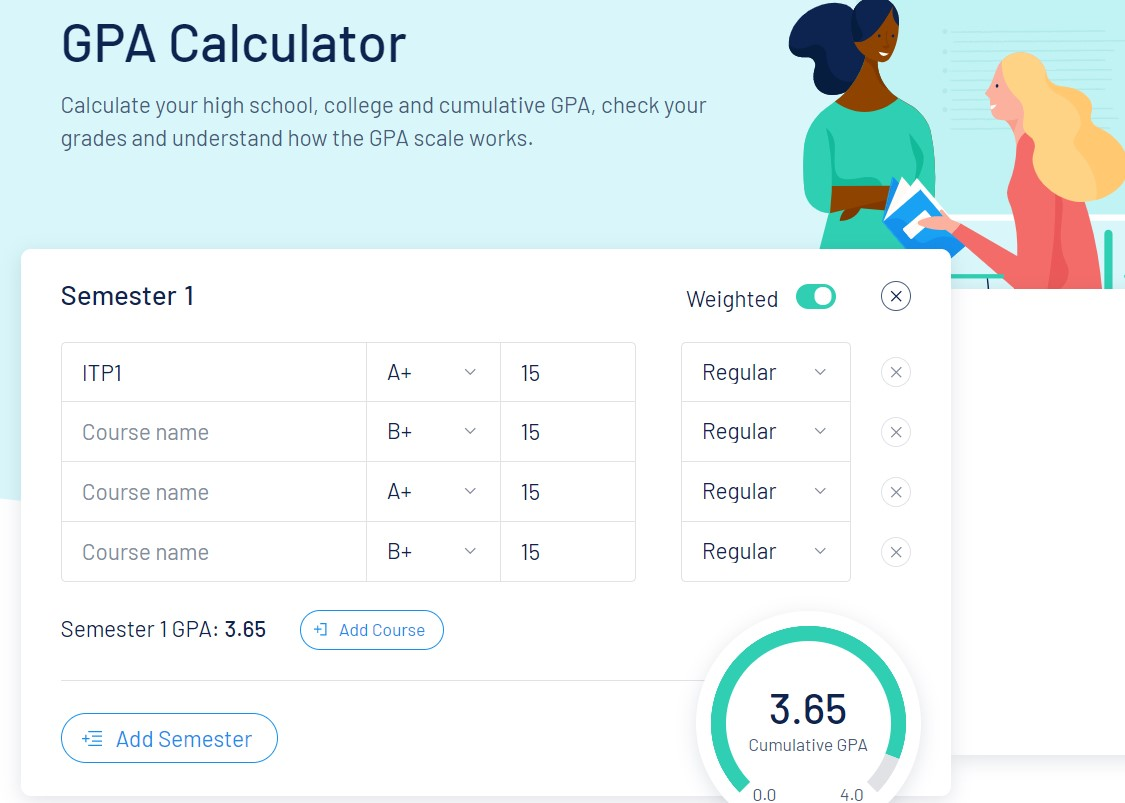
\includegraphics[width=8cm]{gpa-calculator-io}
\centering
\caption{Landing Page Form on gpacalculator.io}
\label{fig:gpa-calc}
\end{figure}
\medskip

\subparagraph{Notable Features}
The tool calculates semester or total cumulative GPA from individual courses, offers different calculators for high school and college and also provides general information about GPA, grades, and different honors.

\subparagraph{Notable Design Choices}
Placement of the input form is very prominent and users are immediately confronted with it when visiting the page. There is no login or data persistence available, and the tool is US-specific.

\paragraph{University of London Portal}

The University of London itself provides access to grades for viewing \cite{uol}. Users can view grades from each semester, broken down by source (coursework vs. exam), as shown in \autoref{fig:uol-grades}

\begin{figure}[H]
\noindent 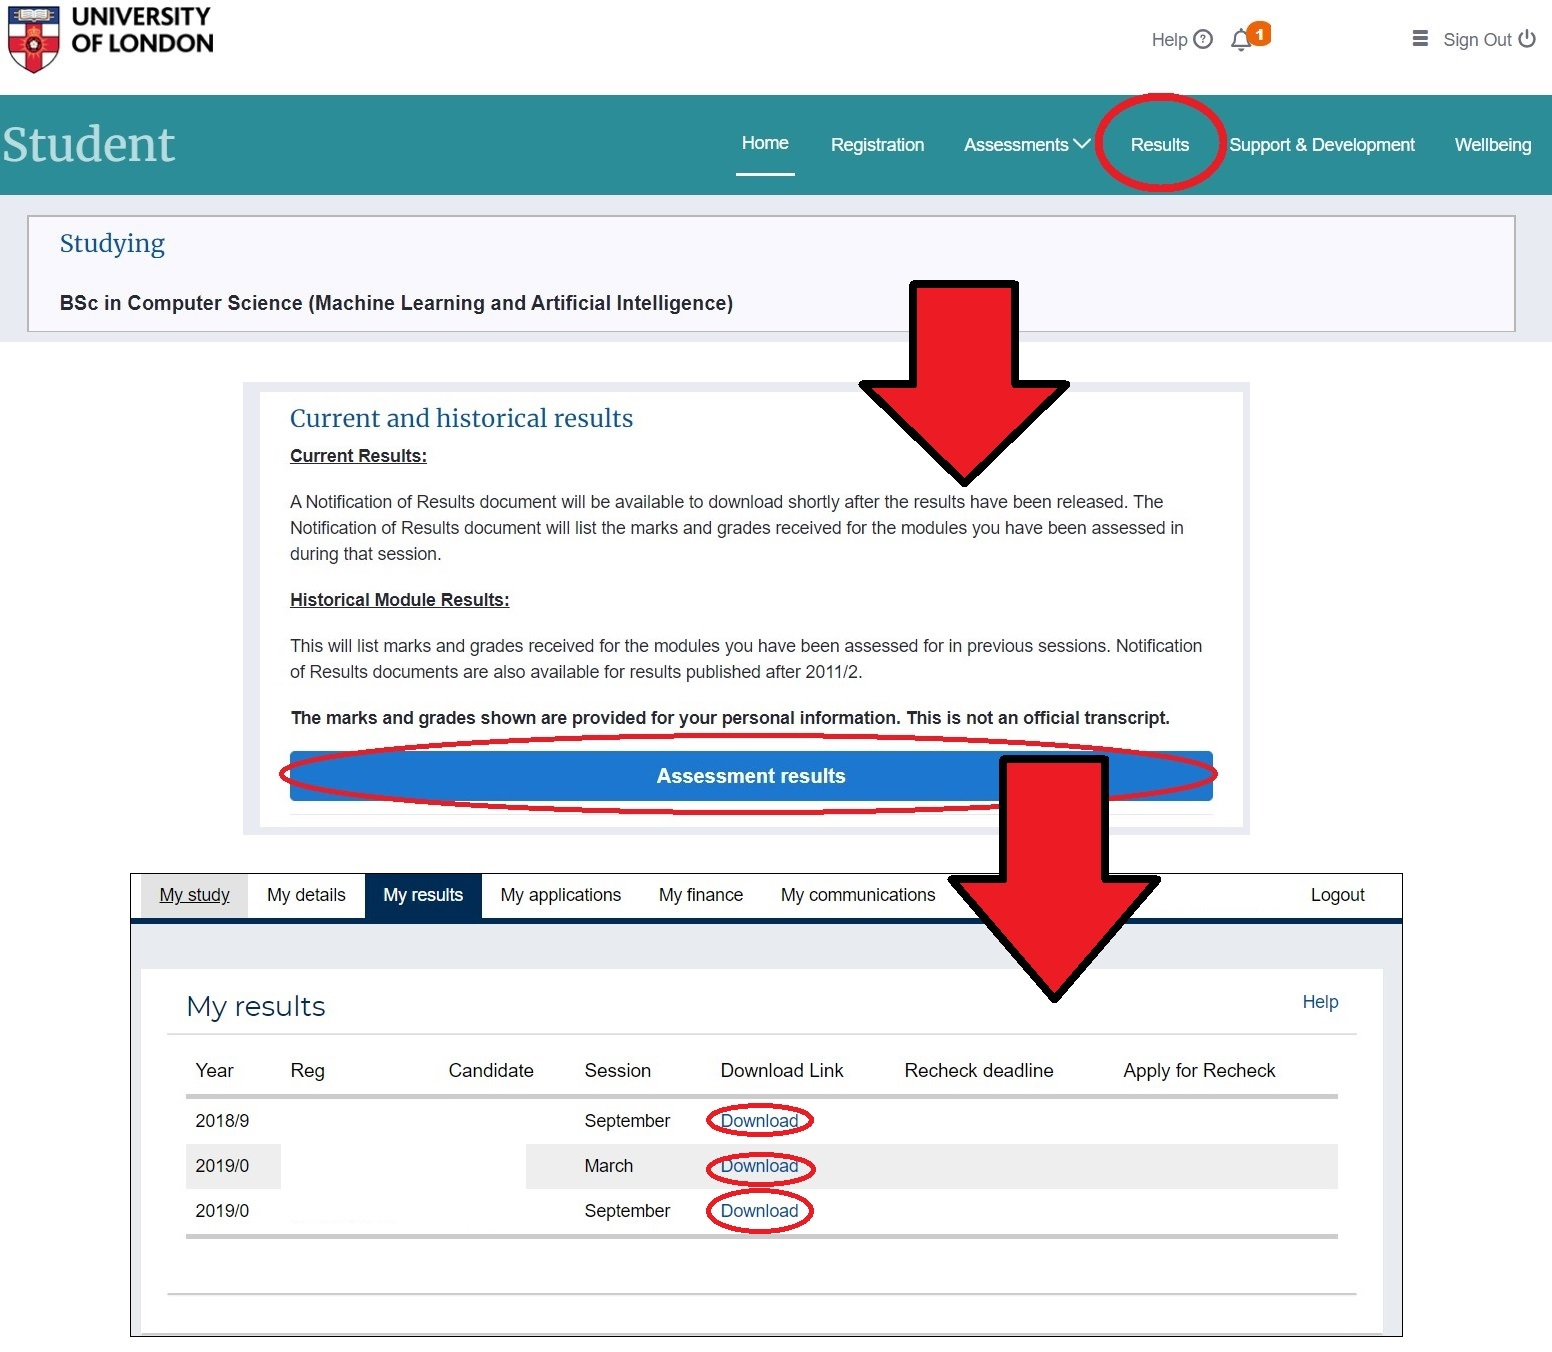
\includegraphics[height=250pt]{uol-buried}
\centering
\caption{Path to find grade download links on University portal}
\label{fig:uol-grades}
\end{figure}

\subparagraph{Notable Features}
The student portal displays official grade results for each semester and shows granular grades for each exam portion separately.

\subparagraph{Notable Design Choices}
Grades are not accessible easily, as they are buried in menus, and there is no centralized display of all grades or cumulative grades. A PDF download is required for all but the most recent grades. The results have the highest level of trustworthiness since they are official.

\subsubsection{Grade Sharing}

We searched the web for 'grade sharing,' 'grade comparing,' 'compare grades to other students,' and other derivatives but found no relevant tools. Glassdoor was suggested as an analogous tool during a brainstorming session and the University of London Slack workspace is known to us through our participation in the degree program.

\paragraph{University of London Slack workspace}

Students at the University of London's online BSc in Computer Science degree use a Slack workspace to collaborate \cite{slack}. Within this workspace, students ehtusiastically share and query grade information following release of results, as shown in \autoref{fig:slack-share}. This workspace is not publicly available.

\begin{figure}[H]
\noindent 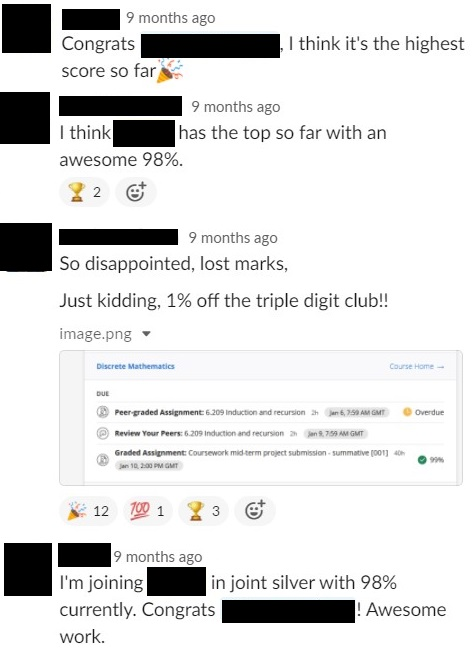
\includegraphics[height=200pt]{slack-share}
\centering
\caption{Students sharing midterm results on Slack}
\label{fig:slack-share}
\end{figure}

\noindent This is the slack space open to all University of London online CS students. There are channels for each course. Grades are sometimes shared in threads after they are released.
\bigskip

\subparagraph{Notable Features}
Slack allows very quick impromptu sharing of grades, however on an irregular basis in bursts during grades season, and the grades are not solicited. Other students can weigh in and react or respond to grades and associated grade queries.

\subparagraph{Notable Design Choices}
Grades reported are usually biased towards students with high grades, or people with low grades who suspect an error in their results.

\subparagraph{glassdoor.com}

Glassdoor is a review and reporting website for employers \cite{glassdoor}. It collects textual reviews and salary data from users. Salary reports are analogous to grade reports in that they are personal information about professional/academic performance that have a similar level of sensitivity.

\begin{figure}[H]
\noindent 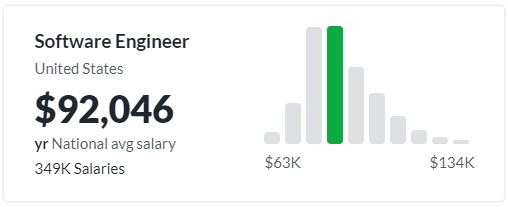
\includegraphics{glassdoor1}
\centering
\caption{Example of data and graph shown on glassdoor}
\label{fig:glassdoor-data}
\end{figure}

\subparagraph{Notable Features}
The site allows users to anonymously collects company reviews and salary information (including job title, locations of position, years of experience). It contains job postings and company profiles with generic information. Users can also submit and collect job interview questions, and the site displays aggregate salary information for specific job titles.

\subparagraph{Notable Design Choices}

Users must submit a salary entry in order to view detailed salary information from other users. The salary collection form is not very prominent and not highlighted on the main site. Users can define their job title, often creating close duplicates of job titles.

\subsection{Comparison of Alternative Solutions}
We abstracted a common set of functionality across these solutions as shown in \autoref{tab:gradestrack} for grade tracking solutions, and \autoref{tab:gradesshare} for grade sharing solutions.

\begin{table}[H]

\begin{tabular}{@{}rcccc@{}}
\toprule
                            & Python Grade Calculator & Degree Planner & gpacalculator.io & UoL Portal \\ \midrule
Track Course Grades         &\checkmark               &\checkmark      &\checkmark        &\checkmark  \\
Calculate Cumulative Grades &\checkmark               &\checkmark      &\checkmark        &            \\
Track Credits               &\checkmark               &\checkmark      &\checkmark        &\checkmark  \\
Granular Grades             &                         &                &                  &\checkmark  \\
Convert Scales              &\checkmark               &                &                  &            \\
Determine Honors Level      &\checkmark               &                &                  &            \\
Persistence                 &\checkmark               &\checkmark      &                  &\checkmark  \\
Shareable                   &                         &\checkmark      &                  &            \\ \bottomrule
\end{tabular}
\caption{Grades Tracking Comparison}
\label{tab:gradestrack}
\end{table}


\begin{table}[H]
\centering

\begin{tabular}{@{}rcc@{}}
\toprule
                                & UoL Slack & glassdoor.com \\ \midrule
Incentivized to submit data     &           &\checkmark     \\
Can compare to others           &\checkmark &               \\
Easy to reference               &           &\checkmark     \\
Aggregates data                 &           &\checkmark     \\
Includes profile on data source &           &\checkmark     \\
\bottomrule
\end{tabular}
\caption{Grades Sharing Comparison}
\label{tab:gradesshare}
\end{table}

\subsection{Market Positioning}
In order to understand our solution's place in the market we need to examine the external factors which might affect the growth and performance of our application.

In the following section we perform both a STEEPLE \cite{bowman_1998} analysis as well as a SWOT \cite{panagiotou_2003} analysis to support identifying the correct market position.

\subsubsection{STEEPLE Analysis}
\textbf{Social}
\begin{itemize}
    \item People tend to be competitive \cite{hutson_2015}.
    \item People may be hesitant to share if their grades are low or they feel they are unfairly graded
\end{itemize}
\textbf{Technological}
\begin{itemize}
    \item Student's participation in the course ensures they will have the hardware necessary to access the website (computer or mobile and internet)
\end{itemize}
\textbf{Economic}
\begin{itemize}
    \item Global audience means any potential efforts to monetize users would be subject to currency risk and local purchasing power.
    \item Enrollment in University of London program and size of other Universities
\end{itemize}
\textbf{Environmental}
\begin{itemize}
    \item Server has energy requirements that will grow with usage
    \begin{itemize}
        \item An increasing number of cloud providers offer solutions that use green energy
\end{itemize}
\end{itemize}
\textbf{Political}
\begin{itemize}
    \item Regulation of data handing is increasing everywhere. This continued trend is exemplified by recent regulations enacted over the past two years:
    \begin{itemize}
        \item Califonia, USA's CCPA
        \item EU's GDPR
        \item Canada's PIPEDA
        \item Japan's APPI 
        \item Brazil LGPD
    \end{itemize}
    Given the global nature of this degree program our application is sensitive to all of these policies and future data protection measures implemented worldwide.
\end{itemize}
\textbf{Legal}
\begin{itemize}
    \item Must comply with local data protection regulations listed above.
\end{itemize}
\textbf{Ethical}
\begin{itemize}
    \item Must handle sensitive data responsibly and transparently
    \item Obligated to maintain a healthy sense of competition and steer away from toxicity and envy
\end{itemize}
\bigskip

\noindent \subsubsection{SWOT Analysis}
\textbf{Strengths}
\begin{itemize}
    \item Knowing you have a relatively high grade could be motivating / encouraging / validating
    \item Validation if your grade was low but many people report similar grades
    \item Highlighting of potentially more challenging courses for future cohorts to allocate more focus and preparation on
    \item Highlighting when many people consider their grades unjustifiably low which may help in organizing a more detailed, thoughtful request to the institution to review the grades or rubric
    \item Motivation to maintain ones standing at or above a certain percentile
    \item Leaderboard aspect "gameifies" grades and gives incentive to submit grades
\end{itemize}
\textbf{Weaknesses}
\begin{itemize}
    \item Data reliability. We have no good way to validate data. We must disincentivize dishonesty and not assume 100\% accuracy.
    \item A small sample size of participants will limit usefulness of averages
    \item Those with poor marks or marks they feel are unjustified will likely be less willing to share
    \item Those who fail or drop out may be unable (depending on integration) or unwilling to participate, which will artificially inflate all grade averages
    \item Without a   representative sample of students, the averaged data, graphs, etc will be skewed and could lead to reduced acceptance or usage of the tool
    \item If we report anonymously, do we also store anonymously? If so then do we provide for the ability to remove data on request?
    \item If the tool is not completely opt-in / crowd-sourced then someone needs to moderate the data insertions and deletions.
\end{itemize}
\textbf{Opportunities}
\begin{itemize}
    \item This project has few real competitors. There are some student created utilities but grade sharing/comparing is outside the scope of those utilities.
    \item The program size will continue to grow for a long time. We haven't reached the maximum number of cohorts and the recent cohorts have grown. The need exists, there just wasn't a reason to make it until now.
    \item If we are the first to make this, we can capture the interested user-base which should be a large moat.
    \item Develop this as with Slack integration so it can naturally link to the community of students that already exists, leveraging the University's policing of that population to being actual students
    \item Add some flags for people to rank their grades. Perhaps they felt the grade was unjustified, or that it was boosted or dragged down by group participants or life events (ie, only receiving a 50\% in a course while feeling stress from COVID)
    \item Provide a field for students to provide short advice to others for each course they provide a grade for
    \item Store the user's grades for visibility of all their courses at once, which if public could be summarized quickly for sharing to others
    \item Provide an overall average per course, per semester, etc to help future students know what to expect and perhaps how much they need to prepare
    \item Provide for grade conversions using various methodologies to non-UK standards
\end{itemize}
\textbf{Threats}
\begin{itemize}
    \item Time. Other student utilities show recognition of value for this type of product. Probably only a matter of time until someone else extends the grade idea in a similar fashion.
    \item Leak or theft of personally identifiable grade and contact information
    \item People could poison the data with dishonest grade reporting
    \item If the tool is completely opt-in / crowd-sourced ...
    \begin{itemize}
        \item ... and we allow the removal of information then perhaps people would remove other people's data
    \end{itemize}
    \begin{itemize}
        \item ... people may impersonate other people along with reporting their real or falsified grades
    \end{itemize}
    \item Loss of integration / changes to any APIs we're using
    \item Data loss - backups
\end{itemize}
\section{Planning and Requirements Gathering}
\subsection{Methodology}
Planning and requirements gathering for this project are based on a classical ``double diamond'' approach. In order to create this proposal, the project team has iterated once internally to gather a potential set of very high-level critical functionality to inform further data gathering. We explored potential topics of interest, narrowed it down to the topic of creating a grade comparison tool for university students, and followingly explored the problem space.

\begin{figure}[H]
    \centering
    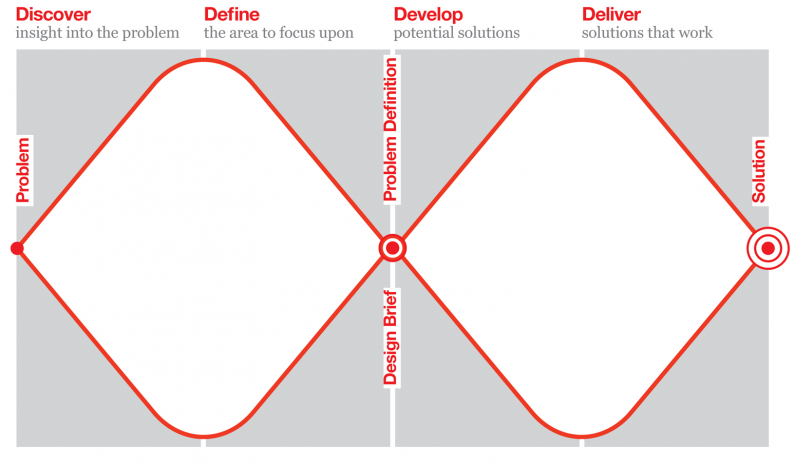
\includegraphics[width=10cm]{images/Double-Diamond-A3-for-publication-A-2000px_1.png}
    \caption{Double Diamond Design Approach}
    \label{fig:doublediamond}
\end{figure}

The reason why we chose the double diamond method is because it is widely used in Design Thinking approaches when project ambiguity is high. The team felt this approach would lead to the highest level of clarity quickly, and would fit into the given timelines by the course schedule and the available capacities of the team.

We considered alternatives such as the Google Design Sprint, but eventually decided not to pursue this as we were not in the need of a 5-day, rapid iteration approach for our solution. We might use it partially during more concrete stages of the project to accelerate progress. We also considered "Research in the wild" (RITW) to find disruptive behaviour-changing ideas, however this approach felt inappropriate as our problem space did not indicate a fundamental challenge to existing technology, but much rather the fulfilment of a basic need of university students often not provided by universities.

\subsection{Discovery}
As background for how we arrived at our final idea, we initially conducted a number of broader exercises to discover potential problem spaces. The team conducted a ``Crazy 8'' exercise in which each team member developed at least 8 new ideas in a time span of a minute for each idea. This laid out a large space of potential ideas the team could work on.

\begin{figure}[H]
    \centering
    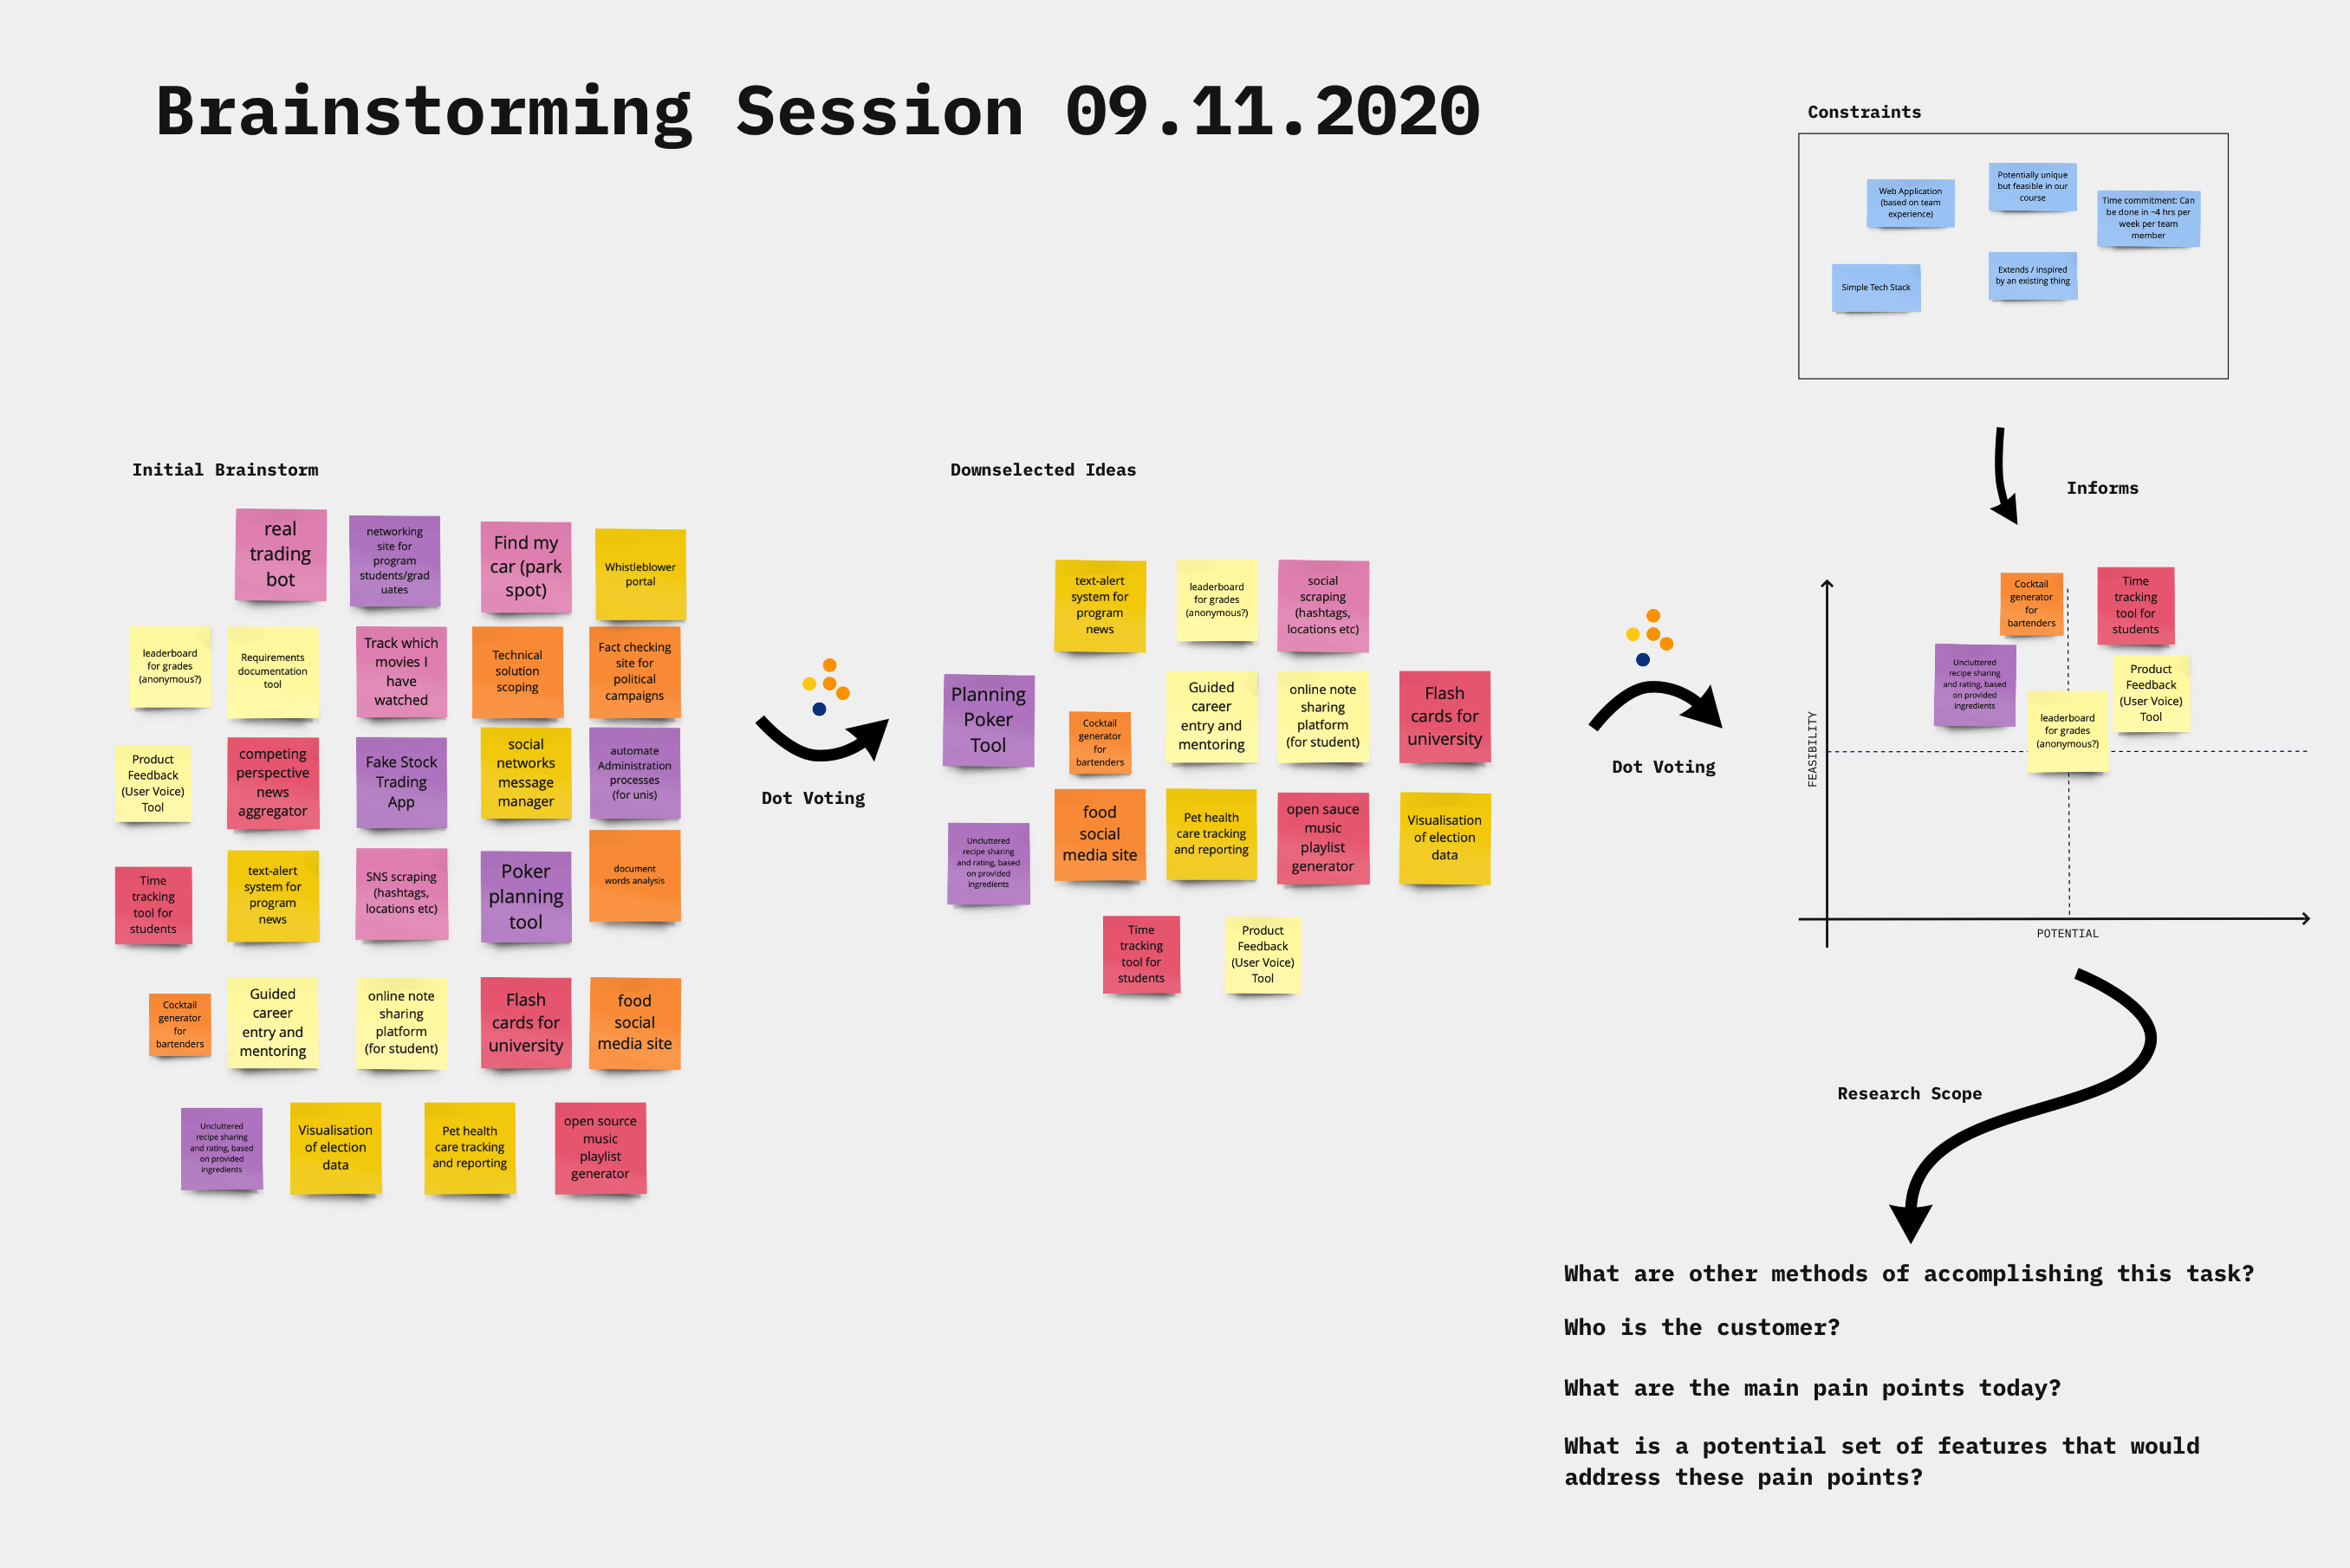
\includegraphics[width=\textwidth]{images/brainstorm.png}
    \caption{Illustration of initial discovery exercise}
    \label{fig:brainstorm}
\end{figure}

Next, we used dot-based voting to narrow down the ideas to those with the highest assumed potential for success and highest interest for the group to further explore. 

Once we had narrowed the ideas down from over 40 to just 5, we decided to explore the potential problem space for each via mind maps, exploring the potential competitive landscape, possible functionality and target users.

\begin{figure}[H]
    \centering
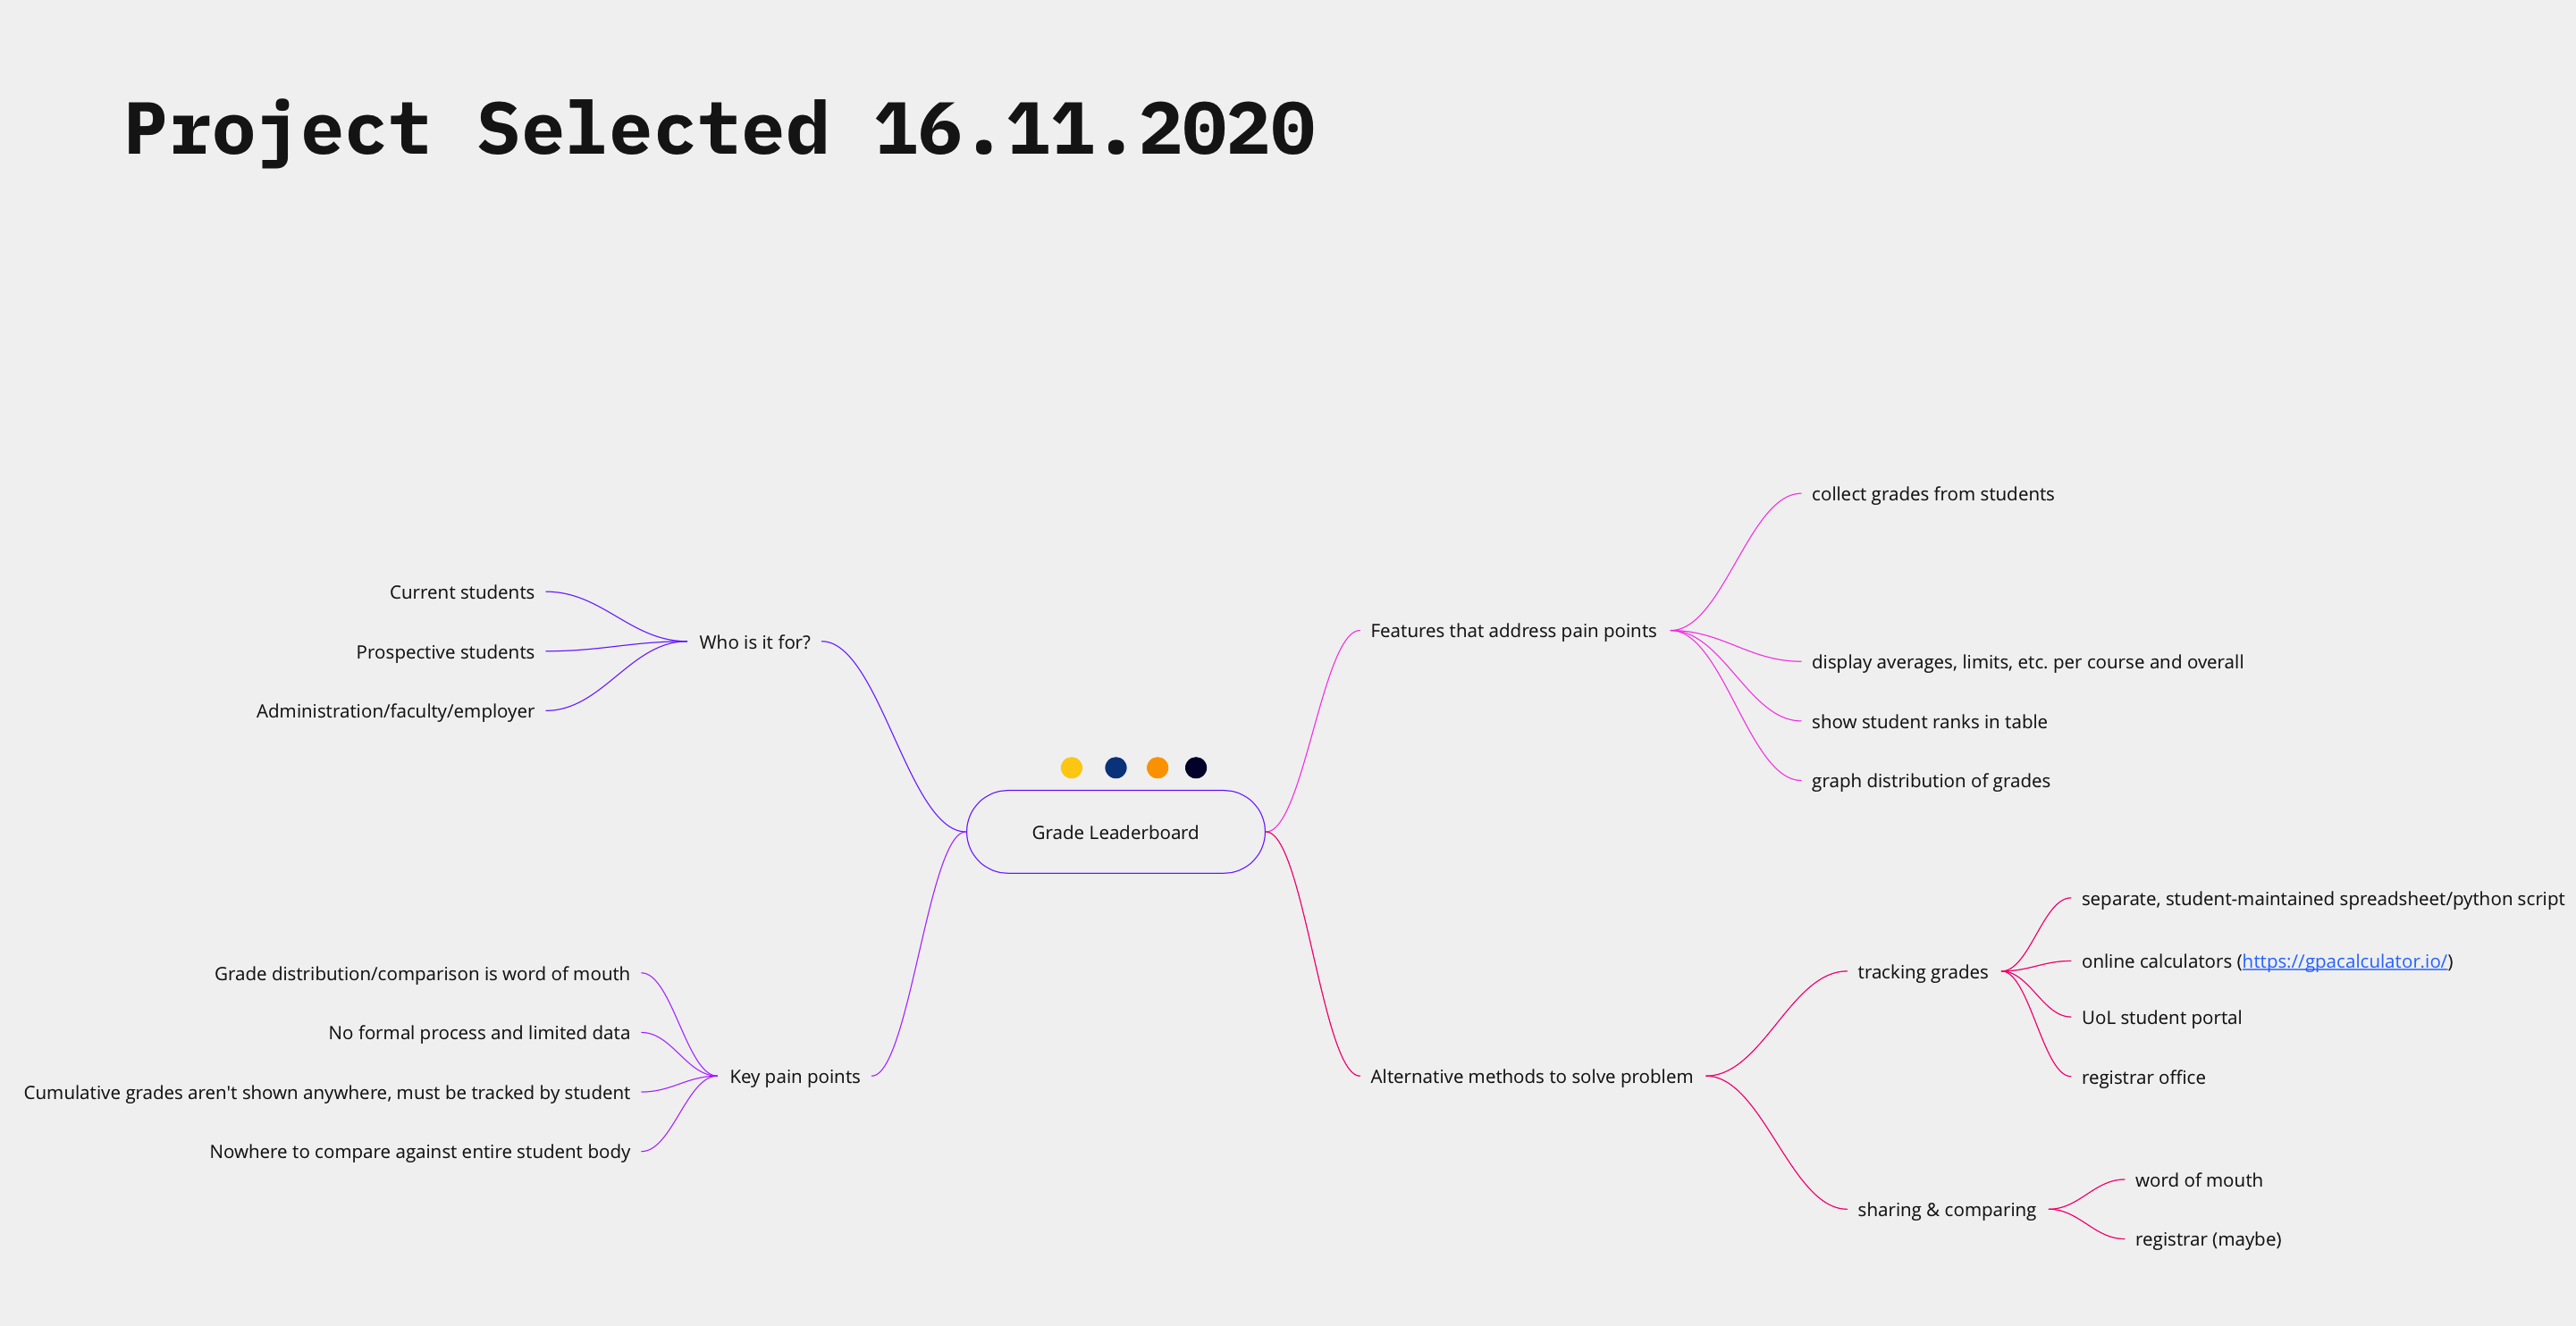
\includegraphics[width=\textwidth]{images/mindmap.png}
    \caption{Mindmap for the winning idea}
    \label{fig:mindmap}
\end{figure}

To further explore the problem space of student grading, we began by brainstorming potential functionality 

\subsection{High-Level Requirements Funnel}

Our approach to gathering requirements will follow these phases, based on the approach for data gathering and requirements analysis described in "Interaction Design" (Sharp et al., 2019).

\begin{enumerate}
    \item \textbf{Data Gathering}: We first use two methods for data recording, namely \textit{questionnaires} and \textit{interviews}. These will serve as initial data input for the project. This will be aided by further desk research to inform the problem space, such as academic papers in the area.
    \item \textbf{Data Analysis}: Analysis of data recorded in this manner will occur based on the analytic framework of \textit{content analysis} and \textit{grounded theory}. We will both develop quantitative and qualitative analysis based on the recorded data. We aim to formulate our \textbf{core hypotheses} around this analysis.
    \item \textbf{Formulate requirements}: Finally, we develop requirements in the form of epics and user stories. To aid this process, we decided to use the frameworks of \textit{contextual inquiry}, which allows us to discover requirements that inspire \textit{joy of use} and \textit{joy of life}, and the 7 product dimensions (Gottesdiener \& Gorman), which allow us to ensure broad coverage of important product attributes.
\end{enumerate}

\subsubsection{Key Research Questions}
As of this report, the team has designed the high-level questions that should be answered by data recording. Our key research questions are listed below. Note that these are not the actual survey questions, but rather the questions we aim to answer through our data recording and analysis.

\begin{itemize}
    \item How do students currently keep track of grades?
    \item How comfortable are students with sharing their grades?
    \item How honest will people be with reporting their grades, anonymously or not?
    \item Why would students want to compare their grades with other students?
    \item Why is this different from just getting the (presumably anonymized) values from the University? Why is this better?
    \item Would there be value in providing automated conversion of grades from the UK standard to standards from other countries?
    \item Does anonymity encourage or hinder contribution to the leaderboards? Does it affect accuracy of reporting?
\end{itemize}

Data gathering will be conducted via an online survey among university students, and interviews will be conducted via online video calls with selected university students.

\subsection{Implementation Approach}

We chose an iterative implementation approach that fits multiple cycles of design, development and user testing from the start of the year until submission of the project by mid-March. This approach envisions that based on completed initial requirements analysis by the end of the year, we can start with short, 2-week cycles of developing the solution. This phase will be closer to a Google Design Sprint in which the team spends focused, full days in developing solutions, implementing prototypes and iterating on the product.

Our project plan attached in full as part of the appendix shows the detailed approach, while \autoref{fig:gantt} shows an illustration of the cycle-based approach until March of 2021.

\begin{figure}[H]
    \centering
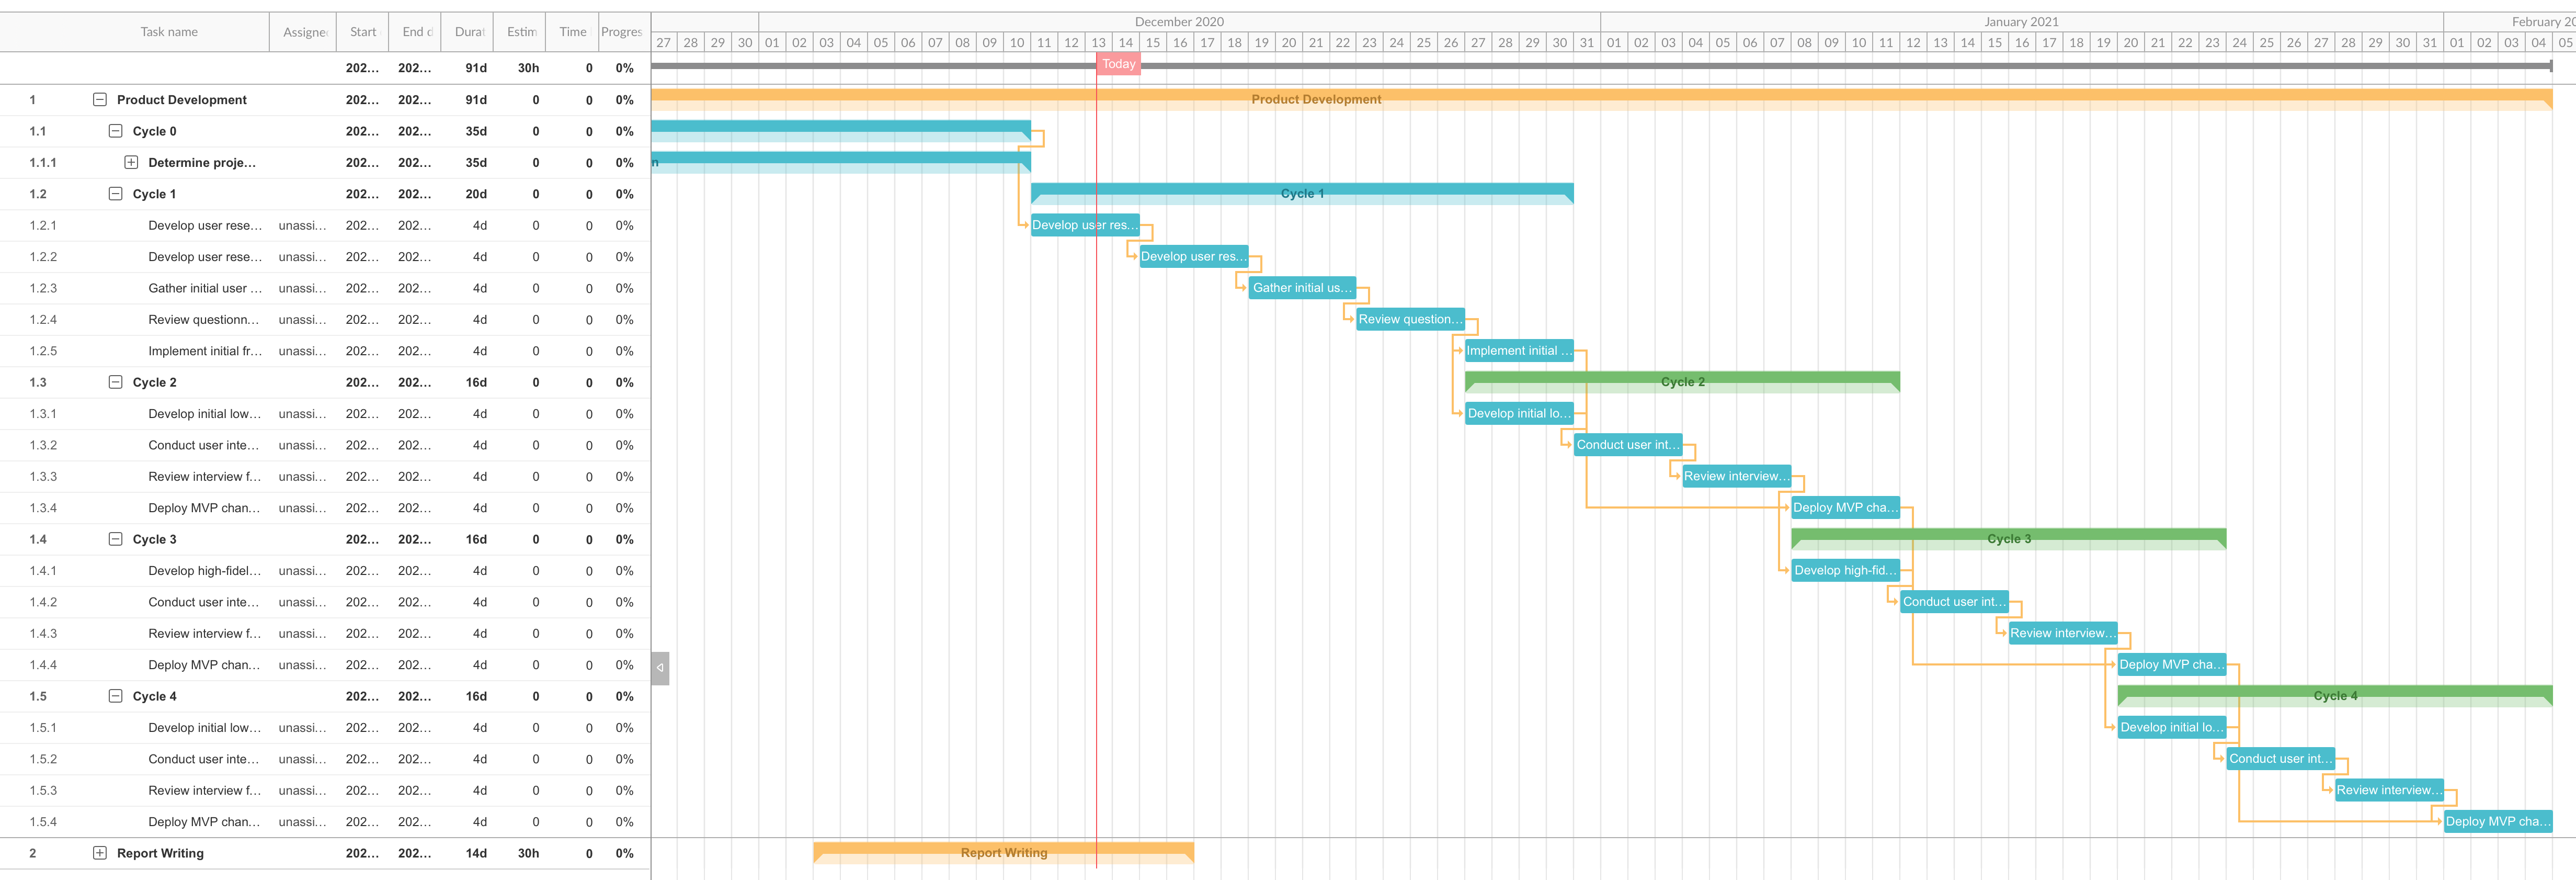
\includegraphics[width=\textwidth]{images/gantt.png}
    \caption{Illustration of the cycle-based project plan}
    \label{fig:gantt}
\end{figure}

\section{Formative Testing and Evaluation}
\subsection{Identifying Users}
In order to identify users, we employ the technique of personas to help identify the right kind of user. We also employ \textit{scenarios} and user fiction to describe the kind of experience we envision for end users.

As a team, we identified the following personas, with detailed personas shown in the figures. The underlying hypothesis is that some users will be more interested in such a tool than others, and do so for different purposes. Our hypothesis is based on the observation that among our own cohort of students in the program, there is a smaller subset of users that are highly active in the student community, generally reporting better grades and mentoring other students, and appreciate some competition. We derive that there must also exist a majority of more casual users who are not as active, but still interested in aspects of grade comparison.

\begin{itemize}
    \item \textbf{Competitive Topper}: Students who are generally top-of-the-class, who enjoy competition and are eager to hit the top of the leader board.
    \item \textbf{Casual Checker}: Students who are not very interested in competitive aspects, but would still like to know where they stand and if they are within the expected range of grades.
\end{itemize}

In order to actually identify users that match these personas, we are including specific questions in this regard in our survey to validate the underlying hypothesis.

\subsection{Testing \& Evaluation Methods}
\textit{Higher marks would require rigorous tests that are insightful and utilise a wide range of metrics to analyse success through different lenses.}


\subsection{Evaluation Type}
The team decided that the most appropriate evaluation type is in \textbf{controlled settings directly involving users}. This means having users peruse the product under observation, describing their experience and providing live feedback. This will be the most efficient approach from a planning perspective.

A further reason this is more appropriate as opposed to \textit{natural settings} is that grades are not something students submit and engage with on a daily basis, hence the opportunities to observe students in this process are rare. This will result in certain downsides of the controlled setting taking precedence, specifically not being able to identify behaviours of users that may occur when unsupervised, which may be central to the grades process. A future iteration may employ screen recording (such as Hotjar) or A/B testing to identify more hidden behaviours.

\subsection{Evaluation Approach}

We will test the produced application at the end of each cycle with 1-3 real student users, recording the outcomes and discussing the results along four categories:

\begin{enumerate}
    \item \textbf{Likes}: What did users enjoy about the product?
        \item \textbf{Problems}: What problems did users encounter while using the product?
            \item \textbf{Ideas}: What are new impulses that users provided while using the product?
                \item \textbf{Questions}: What questions did users ask while using the product?
\end{enumerate}

\section{Prototyping Techniques}
\textit{You should describe your prototype, where strengths in different techniques lie and where they are used. This section should also detail the movement between low- fidelity and high-fidelity techniques, with a view to building the system and the types of technology involved. There should be evidence of iterative design and evaluation steps.}
\subsection{Techniques}
Our strategy towards prototyping will focus on creating a number of low-fidelity prototypes to quickly iterate on, while high-fidelity prototypes will consist of actual software that we can test. We will not create detailed up-front designs or clickable prototypes for the reason that our application's core functionality can easily be communicated with low-fidelity prototypes.

The reasoning for this approach lies in the economic principle of prototyping, which states that the best prototype is one that can demonstrate the possibilities and limitations of a solution in the most efficient manner.

\subsection{Storyboards \& Sketching}
The team developed initial storyboards to illustrate the user journey and make the value proposition tangible. A series of sketches is embedded for the identified personas in \autoref{fig:storyboard_competitive} and \autoref{fig:storyboard_casual}. Based on these storyboards, we learned the following:
\begin{itemize}
    \item The main motivation to log on is likely the need to track grades in a central, easily accessible location that also calculates averages automatically
    \item There are peak times during the year that the tool will see higher usage (e.g. when grades are released)
    \item Students are interested in the distribution of grades on a curve
\end{itemize}

The team will consider these factors in the development of the solution.

\begin{figure}[H]
    \centering
    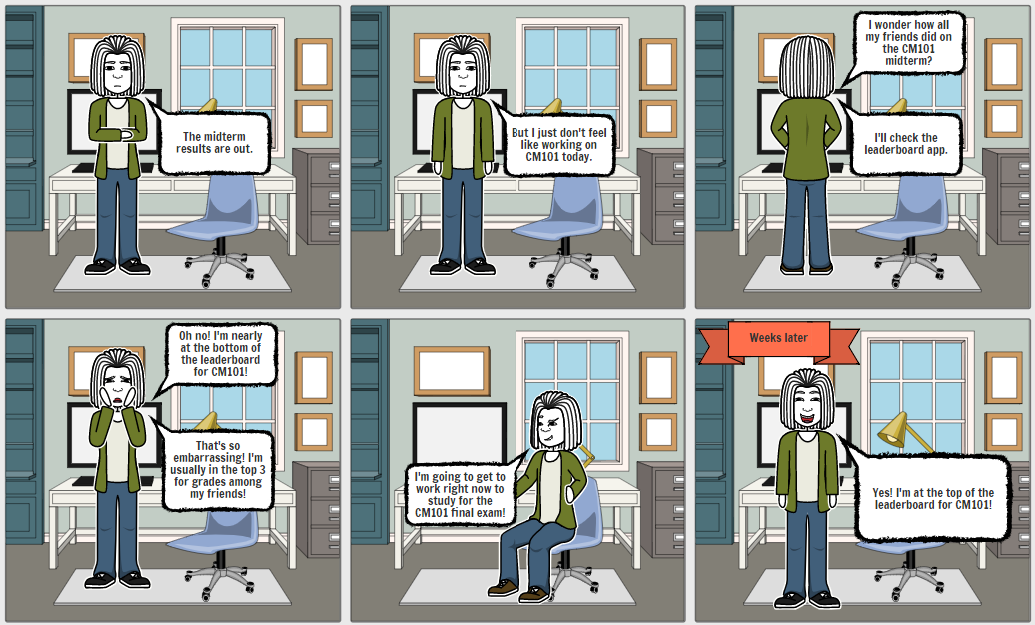
\includegraphics[width=0.95\textwidth]{competitive_topper_1.png}
    \caption{Initial storyboard for the persona ``Competitive Topper''}
    \label{fig:storyboard_competitive}
\end{figure}

\begin{figure}[H]
    \centering
    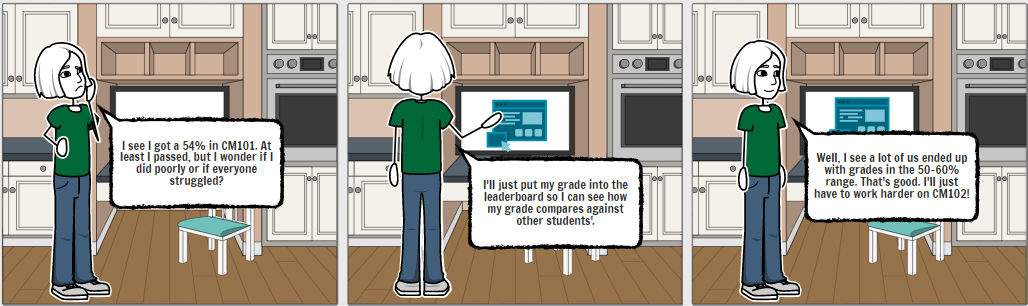
\includegraphics[width=0.95\textwidth]{casual_checker_1.png}
    \caption{Initial storyboard for the persona ``Casual Checker''}
    \label{fig:storyboard_casual}
\end{figure}

\subsection{Wireframes}
To further illustrate how the application will work, an initial wireframe was created to show how an entry page to capture grades might look like. This wireframe was built using a wireframing tool (Balsamiq) and will be iterated on as we move towards building the solution.

\begin{figure}
    \centering
    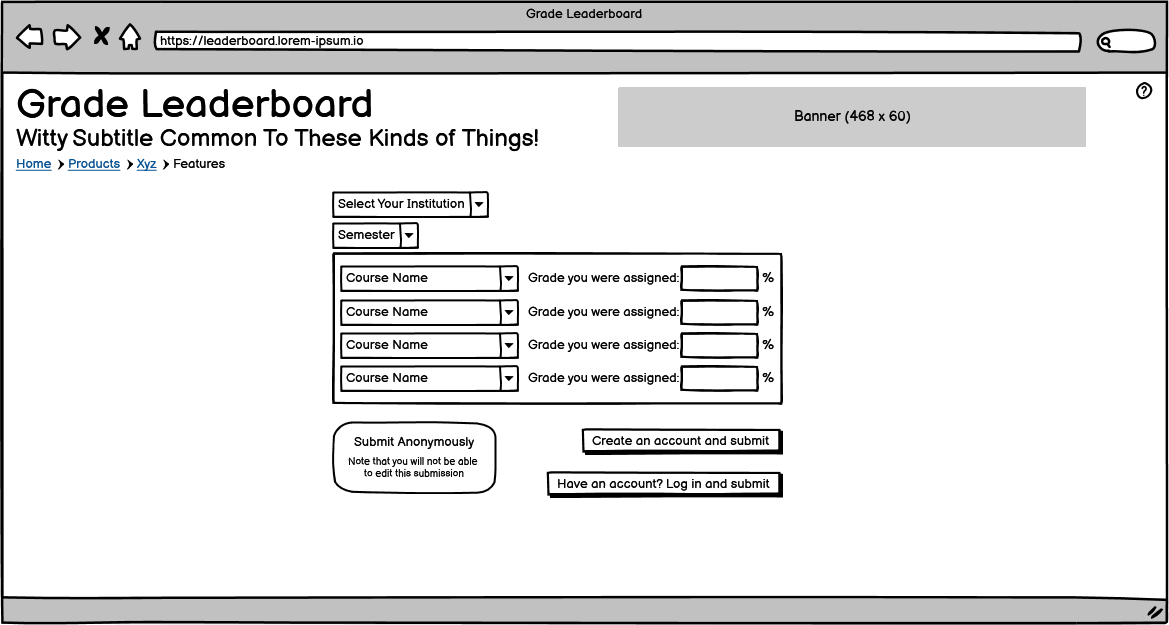
\includegraphics[width=\textwidth]{images/initial_page.png}
    \caption{Early wireframe sketch}
    \label{fig:earlywireframe}
\end{figure}

Based on this very early wireframe, the team identified important questions to consider for further iteration.

\begin{itemize}
    \item Should users enter to see their own overview of grades, or an aggregate?
    \item How might users authenticate into the system?
    \item How does an aggregated view look?
    \item What other information might we need to collect from users?
\end{itemize}

These questions will be further explored during execution of the project.

\section{Evaluation Techniques}
\subsection{Critical Success Factors}
    \noindent When it comes down to success of this project,  following critical factors will be measured. There are five factors and are as follow: reach, coverage, repeat, adoption and rating.  
    Reach is measured by how many students are defined as distinct users who have submitted grades. We define the number of students who registered in the main channel of the collaboration app provided by the university as a total population of students. This critical factor will be set as a percentage of the total student population. ( way of counting total student population may need to be revised) 
    Coverage is measure by how many modules had enough grade submission for meaningful comparison. We consider 5 submission is enough for meaningful comparison. Repeat is measure by how many students have submitted at least two grades over two distinct terms. This program may be used by several institutions and we measure the number of the institution as the adoption. Rating is particularly on users’ feedback on the app include experience with UI. This critical factor is more concerned in long term but not in the initial launch. 

\subsection{Measurement of Success \& Failure}
\noindent We set following measurement to determine if we success or not. There are P0 goals  and strategic goals. P0 goal essentially means what team would like to archive initially to launch of this software and strategic goal is set to be long term goals. \\* \\*

\begin{table}[]
    \begin{tabular}{lll}
                     & P0 Goals                                                                                                   & Strategic Goals                                                                                             \\
    Reach            & 2\% of all student                                                                                         & 5\% of all student                                                                                          \\
    Coverage         & \begin{tabular}[c]{@{}l@{}}66\% of module has enough \\ submission for meaningful comparison.\end{tabular} & \begin{tabular}[c]{@{}l@{}}100\% of module has enough \\ submission for meaningful comparison.\end{tabular} \\
    Repeat           & 10\% of returning student                                                                                  & 30\% of returning student                                                                                   \\
    Adoption         & 1 Program (UoL)                                                                                            & 5 different program                                                                                         \\
    App Store Rating & not apply                                                                                                  & in long-term, 4 stars                                                                                      
    \end{tabular}
\end{table}

\subsection{Results}
\textit{ What works well about the system and where are the fundamental flaws?}

Other points that will likely need to be included as they are included in the course lectures
Version Control - make sure we talk about Github and why we chose it etc
The requirements specifications are included above and coming along
Writing needs to make frequent reference to User Centered Design, as frequent as possible testing and iterations, talk about our heuristics and evaluation methods
Prototyping - are we doing evolutionary or throwaway and why
Sketching or storyboarding?

\bibliography{bib} 
\bibliographystyle{IEEEtran}

\end{document}
